\section{Design}
\label{system_design}

\system{} comprises an overlay network of relays and an oracle that
directs clients to the appropriate relays, as shown in
Figure~\ref{fig:arch}.  \system{}'s relays are TCP proxy servers,
which allow clients to access web content without installing software.
%in contrast, IP layer relays would require clients to install
%software, violating our usability goal.  
\system{} uses the
measurement methods described earlier to learn paths between
clients, relays, and domains; the results are stored at the
oracle.  The oracle uses the data to decide which relay a client in
some location should use for accessing a certain domain while avoiding
a certain country.  The oracle periodically computes paths for many
combinations of client AS, destination, and country.
%A client can then query the oracle to
%determine the appropriate relay to use to avoid a certain country
%en route to a particular destination.
%

%Once the TCP proxies are established, a client needs
%to learn which proxy to use when accessing a given domain.

%\begin{figure}[t]
%\centering
%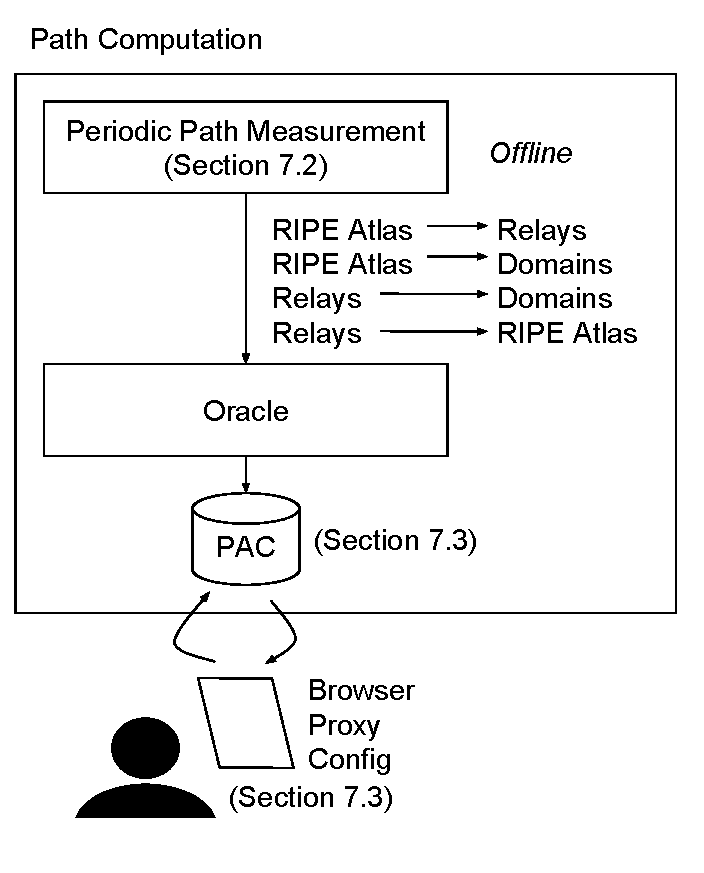
\includegraphics[width=.5\textwidth]{system_overview_updated}
%\caption{\system{} architecture. 1) Paths are computed between clients and relays, 
%relays and domains, relays and clients, and clients and domains.  2) The oracle 
%aggregates all paths.  3)  The oracle generates a PAC file that specifies which 
%domains should be accessed through which relays (based on the measured paths).  
%4) The client configures her browser to use the oracle-generated PAC file.  5) 
%The client's traffic is routed through relays (or direct paths) to access domains, 
%while avoiding a client-specified country.}
%\label{fig:arch}
%\end{figure}

\subsection{Periodic Path Measurement}

All of the paths are measured using {\tt 
traceroute}, which is then mapped to the country level using the same methods as 
described in Section \ref{datasets} and shown in Figure 
\ref{fig:analysis_pipeline}.  The paths we measure are the: forward paths from 
the client to each relay, forward paths from each relay to each domain, forward 
paths from the client to each domain, and reverse paths from each relay to the 
client. 
%Figure \ref{fig:paths} shows the forward and reverse paths when accessing 
%content using relays; the only path we cannot measure is the reverse path from 
%the domains to the relays because we have no 
%vantage point at or near the domain for running traceroute.
\system{} measures paths from clients to relays, clients to domains (servers),
relays to domains, and relays to clients; the reverse path from the domains to the relays 
is challenging to measure due to a lack of vantage points in ASes of
common destinations.  
Despite the inability to measure this part of the
path, it would be difficult for the country being avoided to perform
traffic analysis because it is {\it at most} only on the reverse path 
from the server to the relay. 

\begin{figure}[t!]
    \centering
%    \begin{subfigure}[b]{0.4\textwidth}
        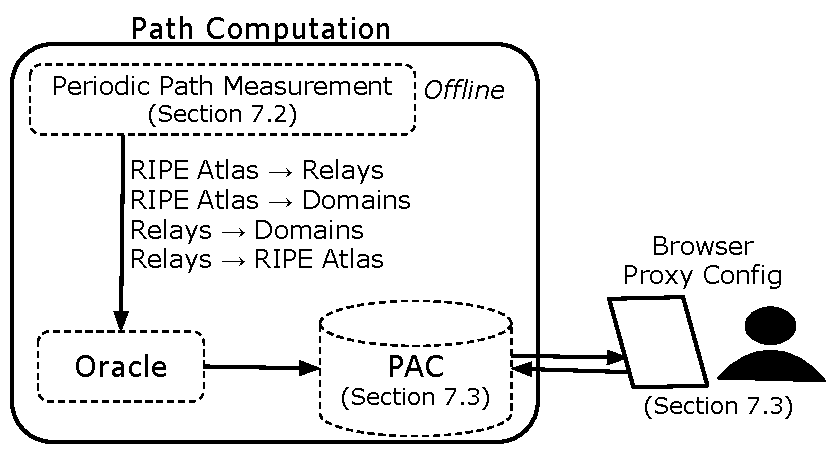
\includegraphics[width=\linewidth]{system_overview_updated-2}
        \caption{\system{} architecture.}
        \label{fig:arch}
%    \end{subfigure}
%    \begin{subfigure}[b]{0.4\textwidth}
%        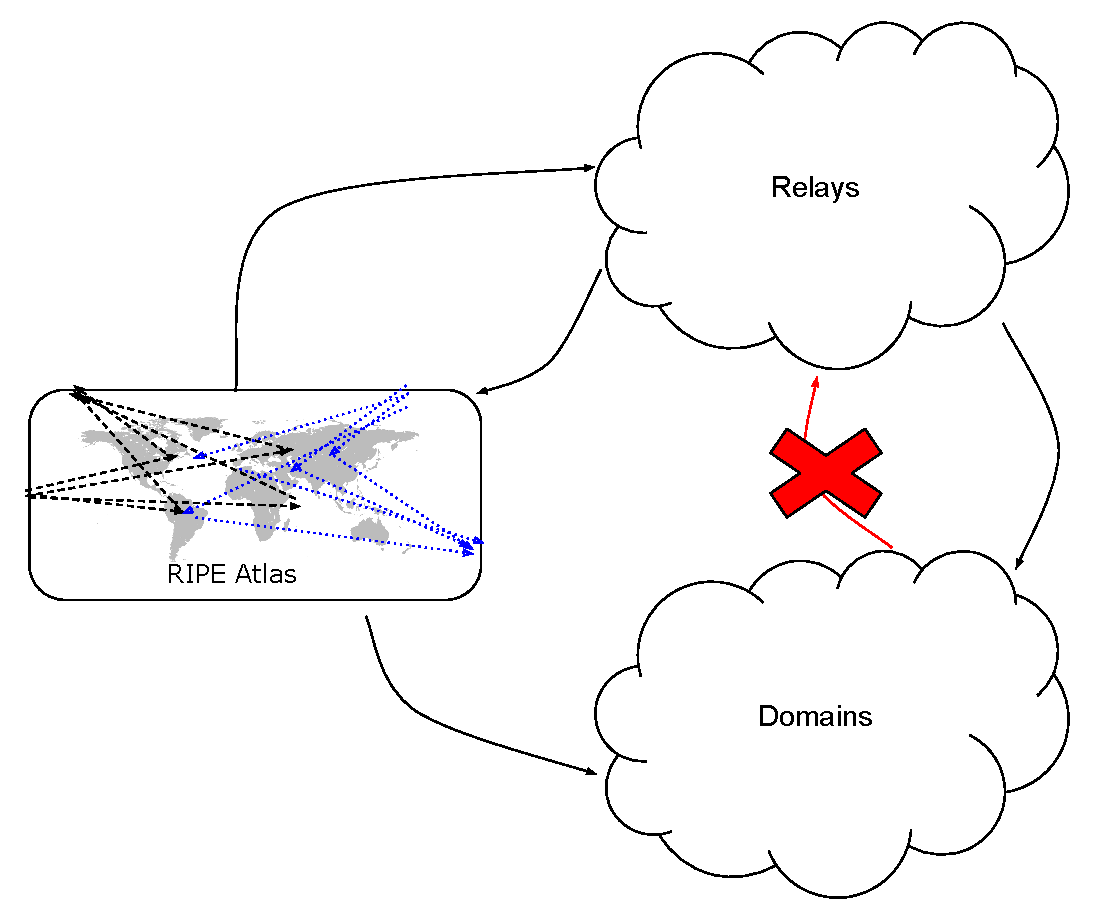
\includegraphics[width=\textwidth,height=7cm]{all_paths}
%        \caption{Paths computed in \system{}.}
%        \label{fig:paths}
%    \end{subfigure}
%    \caption{\system{} architecture, and the path
%      measurements that \system{} periodically computes.}
\end{figure}


\paragraph{Client-to-Relay Paths.} 
To avoid requiring the client to install custom software, \system{}
measures client-to-relay paths from RIPE Atlas probes that serve as 
vantage points for potential client ASes.  \system{} selects probes that
are geographically close the client (\eg, in the same 
country). The oracle triggers the probe to run traceroutes
to each relay.  After collecting the responses, the oracle maps 
the IP-level paths to country-level paths and stores the results.

\paragraph{Relay-to-Client Paths.} The relays perform
traceroutes to the IP addresses of RIPE Atlas probes, which 
represent client ASes.  They then derive country-level paths; the
oracle learns these paths from each relay.  

\paragraph{Relay-to-Server Paths.} Relays perform 
traceroutes to each domain.  As with paths to clients,
relays derive country-level paths and send them to the oracle.

\paragraph{Client to Server Paths.} In a path from a client to a 
domain does not pass through the country specified to avoid {\it by default}, 
then none of the proxies should be used.  
%If a proxy is used, then it may 
%actually be causing the path to traverse more countries
%(unnecessarily).  
These paths are measured using the RIPE Atlas probes in similar
locations as the clients, and the oracle triggers traceroutes from
each of them to each of the domains.  Corresponding country-level
paths are stored at the oracle.

These paths must be re-computed 
as paths may change.  To our knowledge, there has not been any previous work 
on how often country-level paths change; prior work has explored how often 
AS-level paths change.  To measure how often country-level paths change, we 
computed the paths from relays to domains once every two hours and once every 
hour.  Fewer than five paths changed every two hours; the 
results were similar for one-hour increments.  As it takes approximately 30 minutes to 
compute all paths, \system{} re-computes the paths every one hour to incorporate 
the most recent country-level paths.

%\begin{figure}[t]
%\centering
%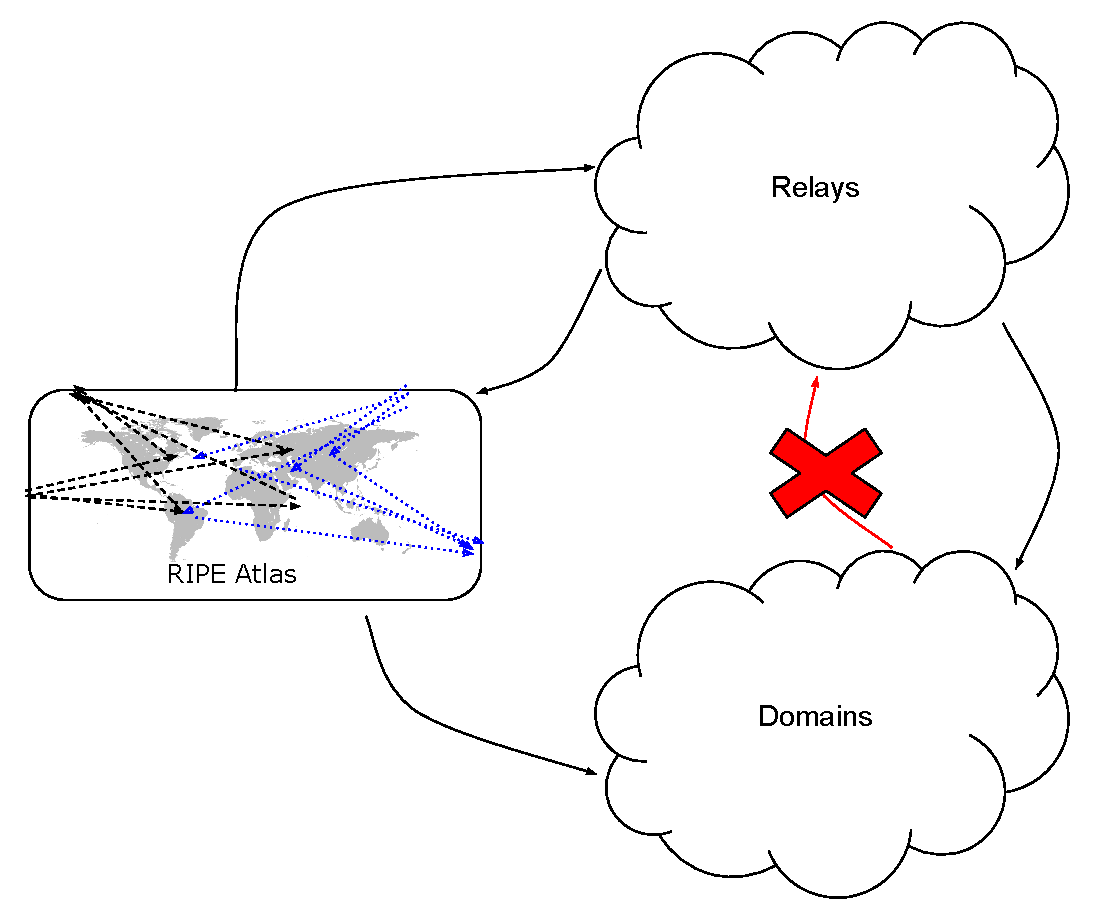
\includegraphics[width=.5\textwidth]{all_paths}
%\caption{The path of a web request through a \system{} relay, to the domain, and back. 
%1) forward path from client to relay; 2) forward path from relay to domain; 3) reverse 
%path from domain to relay; 4) reverse path from relay to client.  \system{} measures 
%all paths except for path 3) due to a lack of vantage points at domain locations.}
%\label{fig:path_components}
%\end{figure}


\subsection{PAC File Generation}
\label{multiplex}
The oracle follows four steps to decide which relay a client should
use to access a specific domain: (1)~If the default path from the
client to the domain does not pass through the specified country, then
do not use any of the relays.  (2)~Otherwise, for all the paths from
the client to the relays, select suitable relays such that the path
does not contain the specified country.  (3)~From this set, if there
is a path from a suitable relay to the domain that does not include
the specified country, then use that relay for that domain.  (4)~If
there is no path from the client through any of the relays to the
domain that does not pass through the specified country, then select
the relay that provides the most avoidance (measured by how many other
domains that avoid the specified country).
\begin{figure}[t]
\renewcommand{\lstlistingname}{Configuration}
\lstinputlisting[label={lst:pac}, language=JavaScript, frame=single,
basicstyle=\footnotesize, caption={Example PAC file.}]{example_pac.pac}
\vspace*{-0.25in}
\end{figure}
The oracle applies this decision process to each domain, which results
in a mapping of domains to relays that can be used to avoid the given
country.  To facilitate automatic multiplexing between relays,
\system{} utilizes Proxy Autoconfiguration (PAC) files, which define
how browsers should choose a proxy when fetching a URL.  In the
example PAC file in Configuration~\ref{lst:pac}, proxy 1.2.3.4:3128
should be used when accessing {\tt www.google.com}, but proxy
5.6.7.8:3128 should be used when accessing {\tt www.twitter.com}.  The
oracle uses the mapping of domains to relays to generate a PAC file,
which specifies which domains should be accessed through which proxy.
The PAC file is published online to a URL of the format
$<$client\_country$>$\_$<$country\_to\_avoid$>$\_pac.pac.  The client
uses this URL to specify their proxy configuration.  Paths are
re-computed every hour, so the contents of the PAC file are also
updated every hour.
% The PAC files are published online, which allows a client to simply
% point the proxy configuration settings to the URL that contains the
% PAC file.

\subsection{Scalability and Fault Tolerance}
Adding relays to \system{} is 
straightforward. Additionally, \system{} is resilient to failures of system components.

\paragraph{Adding relays and oracles.} To add a relay, the system
operator must set up a machine as a proxy server, install the relay
software, and update the oracle's list of relays.  From that point
onward, paths will be computed to and from the new relay, and clients
will begin using the new proxy.  Adding an oracle requires installing
the oracle software on a different machine, and specifying the client
locations handled by that oracle (\eg, one oracle handles clients in
North America and Europe, and another handles clients elsewhere).
Both oracles will publish the PAC files to the same server, which
causes no changes for the client.

\paragraph{Failed relays and oracles.} Unresponsive relays are handled
by the PAC file.  The PAC file allows the oracle to specify multiple
proxies in a sequential order, such that if the the first proxy fails,
then the client users the second proxy (and so on).  This feature can
be used to specify all of the relays that have a path to the domain.
%And future work can include relay replicas that can be used in the
%case that a relay crashes.  
Among other mechanisms, we can detect a failed oracle by determining
that its PAC file is older than one hour.  Detecting a failed oracle
could trigger a backup oracle to re-compute the PAC files
periodically.  Because oracles are stateless, failover is
straightforward.  Without backup oracles, clients can still use the
system when the oracle fails.  The clients will simply be using stale
paths, which are likely (but not guaranteed) to be functional, since
country-level paths change infrequently.


